\documentclass[12pt,journal]{IEEEtran}
\usepackage[letterpaper, margin=0.8in]{geometry}
\usepackage{framed, listings, graphicx, float, amsmath}

\begin{document}

\title{
\includegraphics[width=0.4\linewidth]{figures/rewrite}}

\author{EE149/249A Project Report, Fall 2015

Reia Cho, CJ Geering, Nathaniel Mailoa, Rachel Zhang

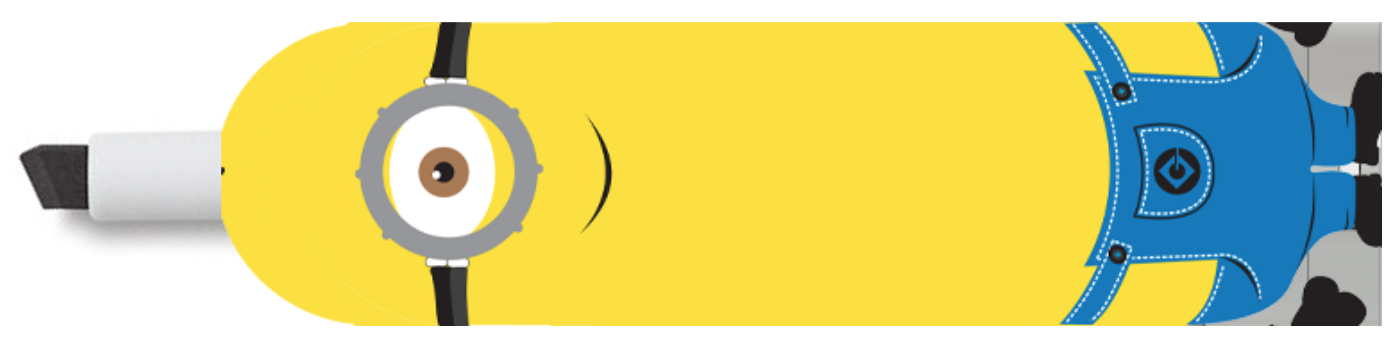
\includegraphics[width=0.45\linewidth]{figures/minion}}


% make the title area
\maketitle



\section{Introduction}
INSERT TEXT HERE

\section{Bill of Materials}
\centering
\begin{tabular}{r|l}
Component & Price \\
\hline
LightBlue Bean & \$30 \\
BNO055 Absolute Orientation Sensor & \$35 \\
Li-Ion 3.7V 150mAh Battery and Charger & \$13 \\
Force Sensor & \$7 \\
Button and LED & \$2 \\
3D Printing & \$2 \\
\hline
Total & \$89 \\
\end{tabular}

\section{System}

\begin{figure}[H]
  \centering
    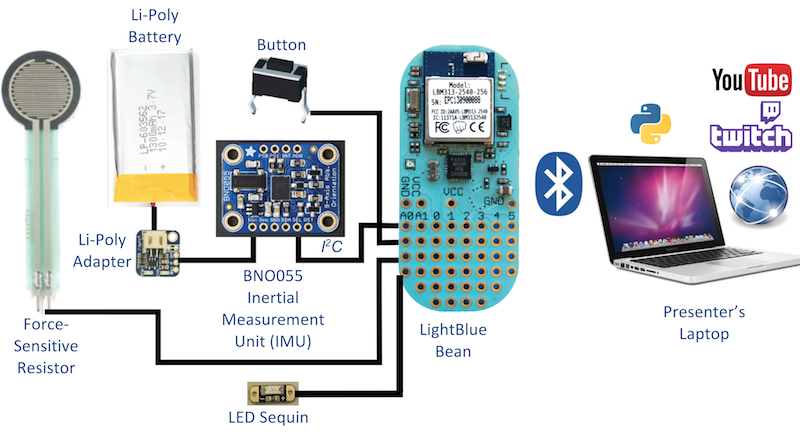
\includegraphics[width=\linewidth]{figures/system}
  \caption{reWRITE system}
  \label{fig:system}
\end{figure}

INSERT TEXT HERE

\subsection{LightBlue Bean}

\begin{figure}[H]
  \centering
    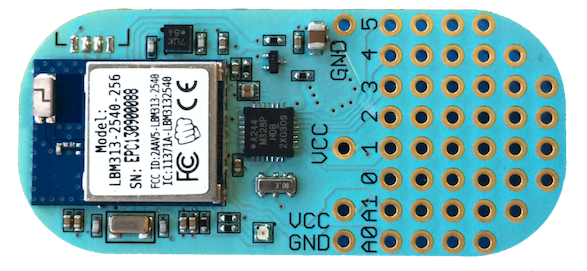
\includegraphics[width=0.8\linewidth]{figures/bean}
  \caption{LightBlue Bean}
  \label{fig:bean}
\end{figure}

For the main controller, we initially chose to use the RedBearLab BLE Nano, but ran into issues with the low level BLE protocol. Because the BLE Nano is typically used to communicate with a smartphone or other BLE modules, we had to develop an XCode project on OSX to use it. There was no high-level software packet on the PC side and the BLE nano also had limited pinouts on the breakout board.
The LightBlue Bean is a more reasonable platform. The Bean has an 8MHz ATMega328p microcontroller, a LightBlue LBM313 Bluetooth Low Energy (BLE) module, an RGB LED, a temperature sensor, and a 3-axis accelerometer. Unfortunately, it does not have a gyroscope, so we still need a separate IMU module. The Bean runs on a 3V CR2032 coin cell and also has a pin that can be used to provide power. The BLE connects to PCs wirelessly and is easy to program because LightBlue provides libraries that simulate serial communication through a virtual serial port. Because the Bean and Arduino Nano have similar functionalities and microcontrollers, we were able to port the Arduino code to the Bean without any compatibility issues.

\subsection{BNO055 Absolute Orientation Sensor Breakout Board}

\begin{figure}[H]
  \centering
    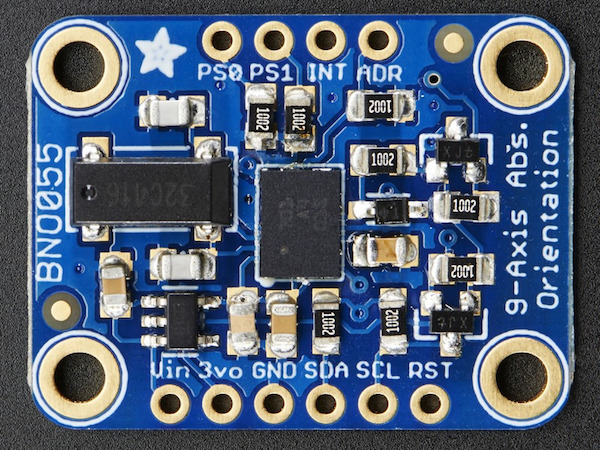
\includegraphics[width=0.6\linewidth]{figures/imu}
  \caption{BNO055 IMU breakout board}
  \label{fig:imu}
\end{figure}
  The BNO055 is a 9-Degree of Freedom Inertial Measurement Unit (IMU) that provides accelerometer, gyroscope, and magnetometer data. Running onboard the 32-bit M0+ microcontroller is the Bosch Sensortec sensor fusion algorithm that combines sensor data for calibration and filtering. This gives us linear accelerations because the sensor fusion accounts for gravity. The processed data is available at a datarate of 100Hz. We also used this device to send Euler angles, which is calibrated against the magnetometer to provide absolute orientation with respect to North. The IMU communicates to the Bean through I2C in the Bean’s analog pins.
  When the device is initially powered, it must be calibrated. Each sensor is calibrated separately by the onboard microcontroller and a register in the device stores the calibration status for each sensor out of 3. The gyroscope is calibrated by keeping the IMU stationary. The magnetometer is calibrated by drawing a figure eight. The hardest sensor to calibrate is the accelerometer. To do so, the IMU must be stationary for a few seconds in various orientations. Overall, the three sensors take about 30 to 60 seconds to calibrate. To help with calibration, we use the Bean’s RGB LED to signify the calibration status using color-coding. Even after the IMU is fully calibrated, it is still not perfect, which we will discuss in the position reconstruction section.
\subsection{Li-Ion Battery}

\begin{figure}[H]
  \centering
    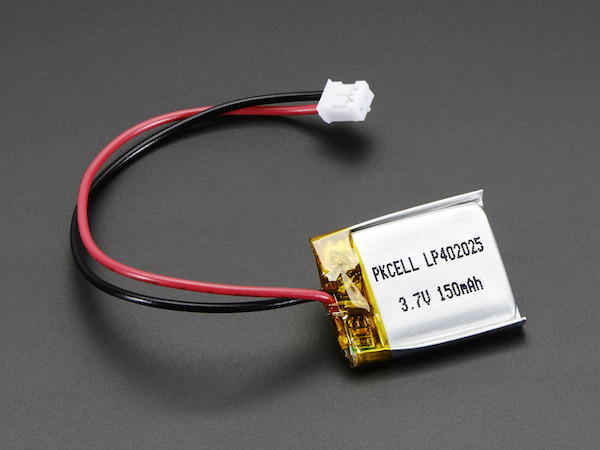
\includegraphics[width=0.6\linewidth]{figures/battery}
  \caption{3.7V 150mAh Li-Ion battery}
  \label{fig:battery}
\end{figure}
  To power our devices, we use a 3.7V 150 mAh Li-Ion battery with a breakout board. This battery was chosen because the small size fits the form factor of the reWRITE. The LightBlue Bean is hooked up to the battery through the IMU board because it needs a source between 3.0 to 3.6V and does not have an on-board regulator.

\subsection{Force Sensor}

\begin{figure}[H]
  \centering
    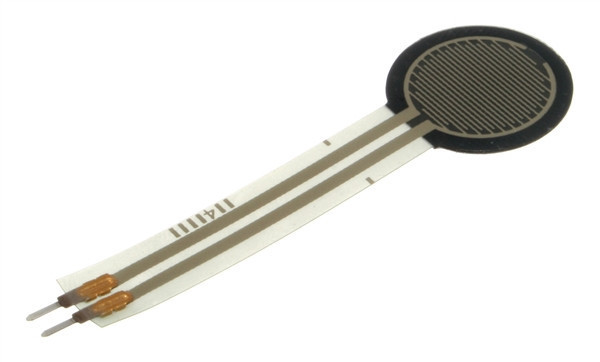
\includegraphics[width=0.6\linewidth]{figures/force-sensor}
  \caption{Force sensor}
  \label{fig:system}
\end{figure}
  To detect when someone is writing with the marker, we attached a force sensor to the back of the marker casing such that the marker pushes against it when it is in use. The force sensor is, effectively, a variable resistor -- about 8 K$\Omega$ when not pushed and about 2 K$\Omega$ when pushed. We used a resistive divider circuit and the digitalRead() function on the LightBlue Bean to determine when the marker was being used. A spring between the force sensor and the marker prevents the marker from constantly pushing against the force sensor.

\subsection{Button and LED Sequin}
  Our last two peripherals were a button and an LED Sequin. The LED Sequin is a tiny module containing a surface-mount LED and resistor which shows whether or not the force sensor is being pushed. The reWRITE also has a small tactile button hooked up to a resistive divider circuit. This lets the user signify that the marker was ready for position calibration (to establish a point of origin). It is also used to clear the plotting canvas in the reconstruction.

\section{Casing}
  For our project, we needed a custom marker casing to attach a force sensor and mount our sensors, peripherals, and microcontroller. Because of cost, ease of use, and endless design possibilities, we chose to 3D print a casing. To make the 3D model, we used Autodesk’s Fusion 360 3D CAD/CAM software and the LulzBot TAZ 5 3D printer. For filament, we initially tried ABS plastic, but we switched to PLA plastic to alleviate warping issues. With used a snap lock design with three components: a end cap, a body, and a front cap. The body of this design was printed in two parts with support material in between to retain structure.
  With the finished print, we used hot glue to fix the force sensor with the spring on the end cap, and secured the marker in the casing with the front cap. Unfortunately, the design does not allow the marker to be capped while it is in the casing.


\begin{figure}[h]
  \centering
    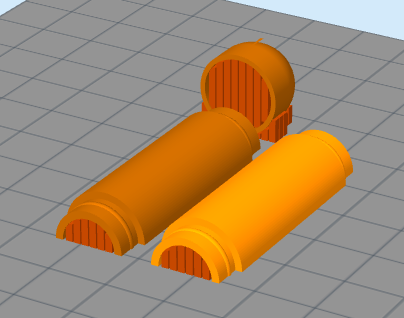
\includegraphics[width=0.6\linewidth]{figures/3d-model}
  \caption{Casing model}
  \label{fig:3d-model}
\end{figure}

\begin{figure}[h]
  \centering
    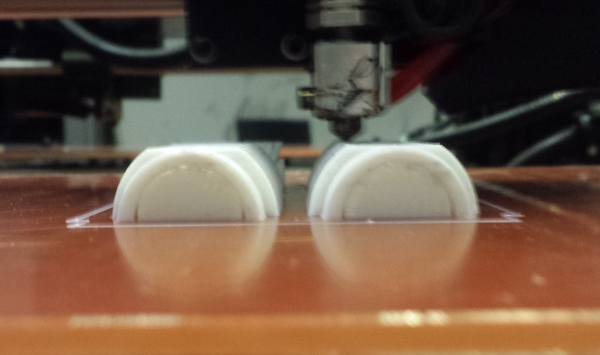
\includegraphics[width=0.6\linewidth]{figures/3d-print}
  \caption{3D printing the casing}
  \label{fig:3d-print}
\end{figure}

\section{Position Reconstruction}
To digitize writing with IMU data, position reconstruction is developed using various methods of post-processing. The reconstruction and plotting code is written in Python with NumPy and MatPlotLib libraries. The code is provided in the appendix.

\subsection{IMU Sensor Data}
	The Bosch IMU provides accelerometer, gyroscope, and magnetometer data. The on-chip Sensortec sensor fusion subtracts the gravity vector to provide linear acceleration. It also uses proprietary algorithms to fuse all nine degrees of freedom to provide more reliable data. The sensor fusion with the gyroscope and the magnetometer provide absolute orientation to North as well as gyroscope stability. From this, we are able to use the Euler angles in position reconstruction. Yaw (rotation about the z-axis) and pitch (rotation about the y-axis) have ranges of 360 degrees, whereas roll (rotation about the x-axis) has a range of 180 degrees.

\subsection{Filtering and Thresholding}
  Once the LightBlue Bean has transmitted the IMU data, we must filter it because the on-chip sensor fusion is not accurate enough for position reconstruction. First, we noted that the IMU calibration was not always perfect. Figure 8a shows the raw data obtained from the IMU on a trial run when it is stationary. As seen by the green line in the plot, the data drifts and gets periodically recalibrated around once every 10 seconds. To solve this issue, we implemented a high pass filter by subtracting the reading away from some mean value computed through a low-pass infinite impulse response (IIR) filter with a very low cutoff frequency. The high-pass filter eliminates this offset as seen in Figure 8b.
  Next, we implemented an IIR low pass filter, which significantly reduces the noise as shown in Figure 8c.
  Lastly, we implemented acceleration thresholding: if the measured acceleration is under a certain threshold, we assume it is due to noise and ignore it. Unfortunately, this thresholding makes it difficult to recognize slow movement. Therefore, we require the user to write with fast movements. The effects are seen in Figure 8d.
\begin{figure}[h]
  \centering
    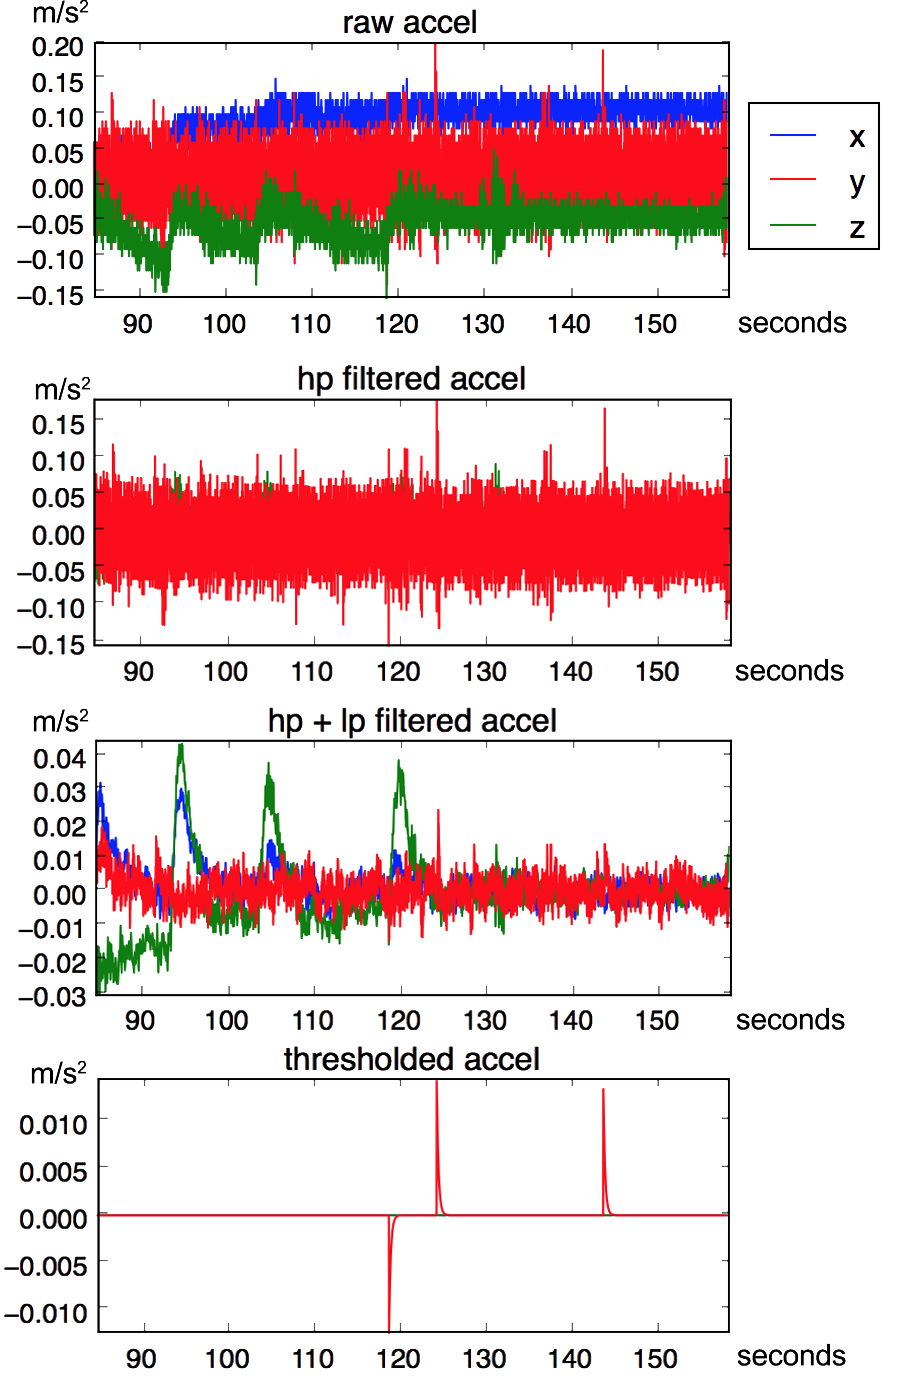
\includegraphics[width=\linewidth]{figures/filtering}
  \caption{(a) Raw data from IMU; (b) Processed with high pass filter; (c) Processed with low pass filter; (d) Thresholded}
  \label{fig:filtering}
\end{figure}

\subsection{Transformation to Fixed Reference Frame}
  Since the acceleration data is provided in the IMU reference frame, we need to perform a change of basis to real world coordinates. The first position recorded is chosen to be the new fixed frame of reference. To perform this basis transformation, we used the Directional Cosine Matrix from [reference here]. $Q_G$ is the coordinates from the fixed reference frame while $Q_P$ is the coordinates from the IMU reference frame.

\begin{figure}[h]
  \centering
    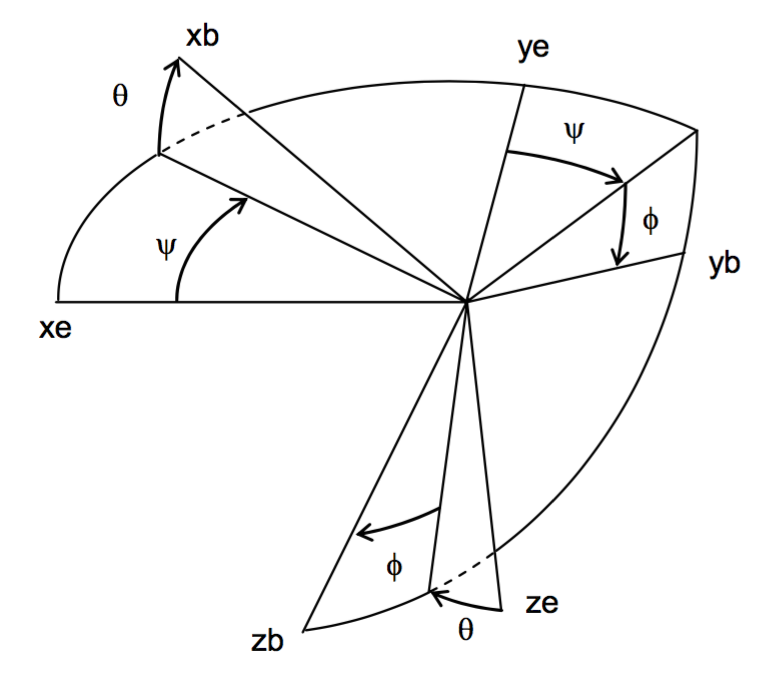
\includegraphics[width=\linewidth]{figures/dcm}
  \caption{Angles corresponding to the DCM [Premerlani and Bizard]}
  \label{fig:vel-adjust}
\end{figure}

\subsection{Velocity Adjustment}
	As we collected acceleration data and tried to reconstruct the position, we discovered that we needed to adjust velocity. When acceleration is near zero for some period of time, it is highly likely that the marker is stationary -- humans typically cannot produce perfectly zero acceleration in a reasonable amount of time. The IMU data is sampled as is imperfect, which causes the velocity to be nonzero as shown in figure [?], which shows velocity reconstruction for a step in the y-axis direction.
	To counter this issue, we assumed that if absolute acceleration is within some small bound for a set time, the velocity should be zero. Then we shift the velocity towards zero by comparing its current value to its value the first and last time the acceleration left the acceleration bounds near zero. Assuming i is the index when the acceleration leaves the bounds and j is the index when the acceleration enters the bounds, the velocity warping formula we used is shown below:
$$v_{\text{adjusted}}[n] = v_{\text{unadjusted}}[n] - \left(\frac{n-i}{j-i}\right)^2 v_{\text{unadjusted}}[j]$$
This algorithm is executed on the 3 axis of movements independent from each other and ensures that the velocity is back to zero when the acceleration is near zero. The resulting velocity is shown in figure [?].

\begin{figure}[h]
  \centering
    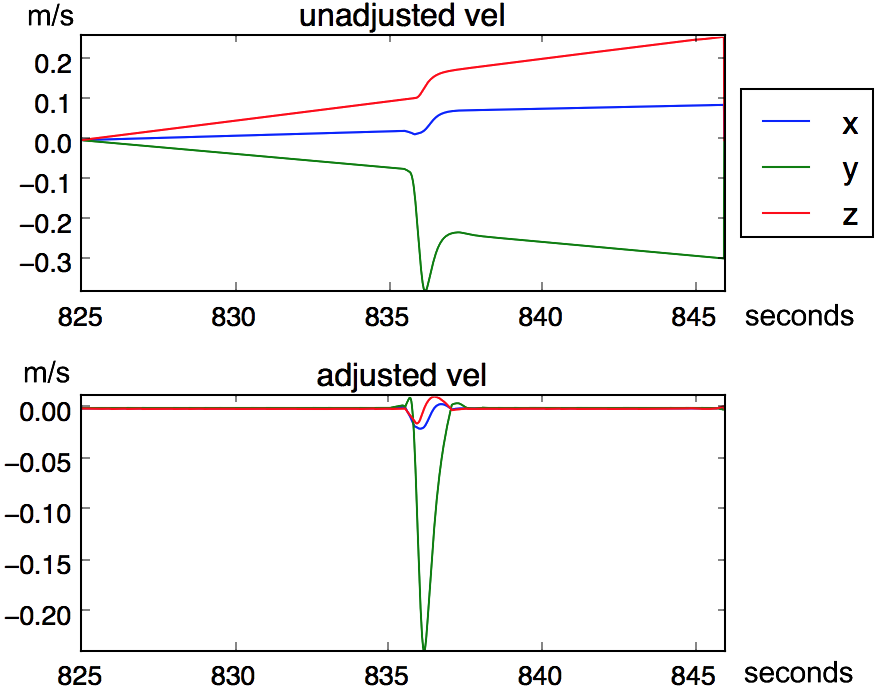
\includegraphics[width=\linewidth]{figures/vel-adjust}
  \caption{(a) Velocity integrated from acceleration data; (b) After velocity adjustment}
  \label{fig:vel-adjust}
\end{figure}

\subsection{Tip Position Reconstruction}
Because the IMU was mounted on the end cap of the marker casing, we used the Euler angles and the distance between the IMU and marker tip to compute the position of the tip. The yaw reading from the IMU did not matter because we draw on a 2D-plane and the marker is assumed to be along the z-axis of the IMU. We calculated that if the reconstructed position of the IMU is $(x,y)$, the tip position is $(x-sin(pitch), y-sin(roll))$.

\subsection{Plotting}
  The position is plotted after reconstruction. We perform the post-processing every 20 data points to reduce latency since NumPy uses vector computations. If the force sensor is turned off during one of the last 20 data points, the plot is updated to include the last stroke. Although we reconstruct position for all transmitted data, we only plot when the force sensor is pressed. We also clear the position plot if button is pressed. 
  
\section{Quantitative Analysis and Scheduling}
	A challenge we encountered was scheduling.The Bean provides the Arduino serial library through a virtual serial port, but it has a limited data rate. Our target data rate was approximately 67 Hz (1 sample every 15 ms). We calculated the worst case execution time (WCET) for each block of code. The first version of our code is shown in [fig ? first CFG] along with the corresponding WCET. Through this quantitative analysis, we discovered that sending data over Serial.println( ) was infeasible to schedule. It took too much time to interpret numbers as actual characters.
	 To make scheduling feasible, we switched from Serial.println to Serial.write( ) to send BLE messages with a 64 byte maximum payload. This sizing allowed us to send five custom data packets per payload. When the IMU was not fully calibrated, we only sent the calibration data to the PC. Once everything was calibrated, we only sent the data. It took about 24 ms to send each payload. However, for every six data packets, one is dropped. We found this to be a reasonable error because the sampling rate was fast enough for our purposes. FIFO buffer concept
	Additionally, the Bean’s RGB LED is controlled by the BLE module instead of the microcontroller, so it takes about 30 ms to set the LED color. But because we do not have a highly customizable scheduler with preemption, we drop two data packets every time we set the LED. This meant that we lost force sensor feedback for that time. To solve this issue, we switched to the LED sequin, which only uses a digitalWrite. 

\subsection{Custom Data Packets}
Each of our custom data packets contains 5 readings of 12 bits. The purpose of each bit can be seen in figure [?]. The valid bit is used to signify that the IMU is fully calibrated. Three bits are assigned to buttons and the force sensor depending on their on or off status. Each axis of acceleration has 12 bits encoded which adds up to 36 bits and allows for an acceleration range of -20.48 to 20.47 $m/s^2$. Sixteen bits are assigned to each axis of the Gyroscope to allow for a range of -180 to 180 degrees with 2 decimal places. The last eight bits are to help with detecting packet loss.

\section{Mode of Operation}
	reWRITE can be modeled okay this is not how the sentence should be phrased but I can’t think of a different way to say it right now by the hierarchical state machine in figure [?]. 
When reWRITE is turned on, it enters the ‘Calibration’ state. In this state, the IMU calibrates the accelerometer, gyroscope, and magnetometer, printing each level of calibration. As soon as all three sensors are calibrated, reWRITE preemptively transitions and enters the ‘Button’ state. Here, it waits for the user to press the button before starting position reconstruction. Once the button is pressed, reWRITE enters the ‘Data’ state. The nested state machine in ‘Data’ is also a hierarchical state machine. In ‘Data’, the system constantly receives new data and plots the reconstructed position. It performs calculations and plots by utilizing synchronous composition of state machines in the ‘Active’ state. One of the synchronous state machines executes the velocity calibration [reference to that section of report?] when the guard evaluates to true replace with what the guard actually is?. Simultaneously, the other state machine plots the position when the marker presses the force sensor. 

\section{Acknowledgements}
We would like to acknowledge the following individuals for their support and contribution in this project.
\begin{itemize}
\item Trung Tran, \textit{National Instruments}
\item Prof. Sanjit Seshia, \textit{UC Berkeley}
\item Matthew Weber, \textit{UC Berkeley}
\item Eric Kim, \textit{UC Berkeley}
\item Casey Rogers, \textit{UC Berkeley 3D Modeling Club}
\end{itemize}

\begin{thebibliography}{1}
\bibitem{PB} Premerlani, W., Bizard, P.: Direction cosine matrix	IMU: theory. http://gentlenav.googlecode.com/files/DCMDraft2.pdf
\end{thebibliography}

\newpage
\onecolumn

\section{Appendix 1: LightBlue Bean code}
\small{
\lstinputlisting[language=C,frame=single,breaklines=true]{stream_data.ino}
}

\section{Appendix 2: Python code}
\small{
\lstinputlisting[language=Python,frame=single,breaklines=true]{draw.py}
}

\end{document}



